\section{Auswertung}

\subsection{Auswertung der Simulationsdaten}
Da die Simulationsdaten Events enthalten, welche für die Auswertung nicht relevant sind, werden diese zunächst selektiert. Die Verteilung der Selektionsvariablen sind in Abbildung \ref{fig:Cuts_sim} abgebildet.
\begin{figure}
    \centering
    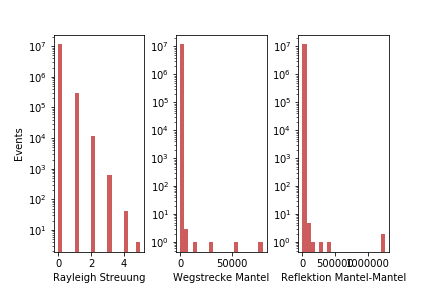
\includegraphics[width=0.5\textwidth]{plots/cuts_sim.pdf}
    \caption{Verteilung der Selektionsvariablen (von links nach rechts): Anzahl Rayleigh-Streuungen, Wegstrecke im Mantelmaterial, Reflektion an der Mantel-Mantel-Grenzfläche.}
    \label{fig:Cuts_sim}
  \end{figure}
  \FloatBarrier
Photonen, welche in der Faser gestreut werden, können nicht mehr durch die in Kapitel \ref{theorie} gefundenen Gleichungen beschrieben werden. Aus diesem Grund werden Ereignisse, deren Anzahl an Rayleigh-Streuungen (\textit{rayleighScatterings}) größer als Null ist, verworfen.
Des Weiteren sollen im Folgenden zwischen Photonen unterschieden werden, welche sich lediglich im Kern bewegen und welche, die in den Mantel reflektiert werden. Die Ersten werden im Folgenden als Kernphotonen bezeichnet, während die Photonen, welche in den Mantel eindringen, Mantelphotonen genannt werden.
Zu den Mantelphotonen zählen die Photonen mit einer Wegstrecke im Mantelmaterial (\textit{length\_clad}) und einer Anzahl an Reflektionen an der Mantel-Mantel-Grenzfläche (\textit{reflClCl}) größer Null. \\

Im Anschluss wird für alle Photonen der Winkel $\theta$ zwischen der $x$-Achse der Faser und ihrer Wegstrecke bestimmt. Anhand von Abbildung \ref{fig:Geometrie} kann der Zusammenhang
\begin{align}
    \vec{p}\vec{e}_{\mathrm{x}} &= |\vec{p}||\vec{e}_{\mathrm{x}}| \cos(\theta) \\
    \Leftrightarrow \theta &= \arccos(p_{\mathrm{x}})
\end{align}
hergeleitet werden. Die Verteilung von $\theta$ für die Kern- und Mantelphotonen ist in Abbildung \ref{fig:theta_sim} dargestellt.
\begin{figure}
    \centering
    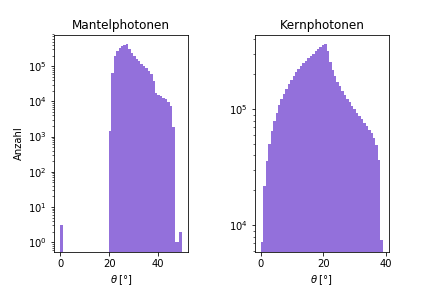
\includegraphics[width=0.5\textwidth]{plots/theta_sim.pdf}
    \caption{Verteilung vom Winkel $\theta$, welcher den Winkel des Photons zur $x$-Achse beschreibt, für die Kern- und Mantelphotonen.}
    \label{fig:theta_sim}
\end{figure}
\FloatBarrier
Die Kernphotonen weisen eine unsymmetrische Verteilung um etwa $\SI{20}{°}$ auf, wobei in dem Bereich oberhalb des Maximums weniger Photonen zu finden sind. Es werden Werte zwischen $\SI{0}{°}$ und $\SI{40}{°}$ angenommen. Die Verteilung der Mantelphotonen hingegen beginnt bei einem Winkel von etwa $\SI{20}{°}$ Grad und nimmt auch Werte etwas oberhalb von $\SI{40}{°}$ an.\\

Mit Hilfe der Histogramme wird das Verhältnis von Kern- und Mantelphotonen für jeden Winkel $\theta$ bestimmt, indem die Anzahl an Einträgen der Mantelphotonen pro Bin durch die Anzahl an Kernphotonen dividiert wird. In Abbildung \ref{fig:ratio_sim} sind die Verhältniswerte in Abhängigkeit von $\theta$ zu erkennen.
\begin{figure}
    \centering
    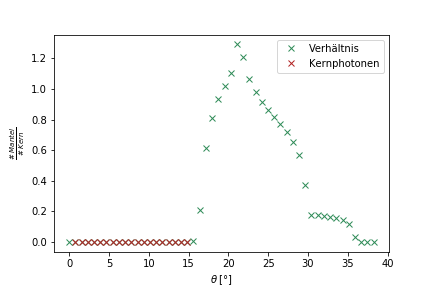
\includegraphics[width=0.5\textwidth]{plots/ratio_sim.pdf}
    \caption{Verhältnis von Kern- und Mantelphotonen in Abhängigkeit vom Winkel $\theta$ (grün). In rot sind die Winkelbereiche gekennzeichnet, in denen nur Kernphotonen auftreten.}
    \label{fig:ratio_sim}
\end{figure}
\FloatBarrier
Ein besonders starkes Vorkommen von Mantelphotonen ist in einem Winkelbereich von etwa $\SI{15}{°}$ bis $\SI{30}{°}$ zu erkennen, wobei sich das Maximum bei einem Winkel von etwa über $\SI{20}{°}$ befindet.

Verhältnisse von Kern- und Mantelphotonen mit dem Wert Null weisen auf Winkelbereiche hin, in denen lediglich Kernphotonen auftreten. Diese Bereiche sind in Abbildung \ref{fig:ratio_sim} mit der Farbe rot gekennzeichnet und treten für Winkelbereiche unterhalb von
\begin{align*}
    \theta_{\mathrm{just core, max}} = \SI{14.82}{°}
\end{align*}
auf. \\

Der minimale Abstand $r_{\mathrm{min}}$ der Kernphotonen zur $x$-Achse kann über den Abstand windschiefer Geraden bestimmt werden. Hierzu wird der Weg des Photons mit der Gleichung
\begin{align}
    p(t) = \left(\begin{array}{c} x\_start \\ y\_start \\ z\_start \end{array}\right)
        + t \left(\begin{array}{c} px\_start \\ py\_start \\ pz\_start \end{array}\right)
\end{align}
und die $x$-Achse mit
\begin{align}
    a(s) = \left(\begin{array}{c} 0 \\ 0 \\ 0 \end{array}\right)
        + s \left(\begin{array}{c} 1 \\ 0 \\ 0 \end{array}\right)
\end{align}
parametrisiert.
Mit Hilfe des orthogonalen Vektors auf die Stützvektoren
\begin{align}
    \vec{n} = \vec{p}\; \times \; \vec{e}_{\mathrm{x}} = \left(\begin{array}{c} 0 \\ pz\_start \\ -py\_start \end{array}\right)
\end{align}
kann die Hilfebende
\begin{align}
    E = pz\_start \cdot y\_start - py\_start \cdot z\_start
\end{align}
konstruiert werden. Der Abstand ist dann schlussendlich durch
\begin{align}
    r_{\mathrm{min}} = \frac{|pz\_start \cdot y\_start - py\_start \cdot z\_start|}{\sqrt{pz\_start ^2 + py\_start^2}}
\end{align}
gegeben. Die Verteilung von $r_{\mathrm{min}}$ ist Abbildung \ref{fig:rmin_sim} zu entnehmen.
\begin{figure}
    \centering
    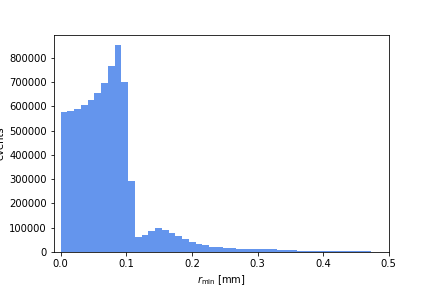
\includegraphics[width=0.5\textwidth]{plots/rmin_sim.pdf}
    \caption{Verteilung des minimalen Abstandes $r_{\mathrm{min}}$ zwischen Photonen und $x$-Achse.}
    \label{fig:rmin_sim}
\end{figure}
\FloatBarrier
Es lässt sich ein gleichmäßiger Anstieg der Verteilung bis zu einem Wert von $r_{\mathrm{min}} \approx \SI{0.1}{mm}$ erkennen, wo die Werte steil abfallen.
Anhand von $r_{\mathrm{min}}$ werden die Kernphotonen auf Daten zugeschnitten, deren $r_{\mathrm{min}}$ kleiner als der Radius der Kernfaser von $\SI{0.1}{mm}$ ist.\\

Zur Bestimmung des mittleren Abstandes pro Winkel werden die $r_{\mathrm{min}}$ in Abhängigkeit von $\theta$ in Abbildung \ref{fig:Hist_rmin_sim} in einem zweidimenesionalen Histogramm aufgetragen.
\begin{figure}
    \centering
    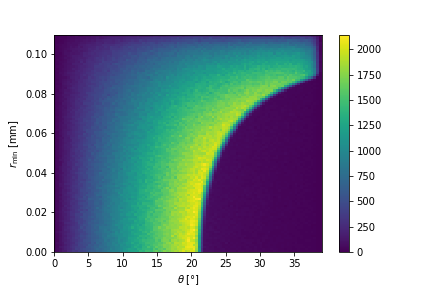
\includegraphics[width=0.5\textwidth]{plots/hist_rmin_sim.pdf}
    \caption{Zweidimenesionales Histogramm der $r_{\mathrm{min}}$ in Abhängigkeit von $\theta$.}
    \label{fig:Hist_rmin_sim}
\end{figure}
\FloatBarrier
Entlang der Achse eines jeden Winkels werden die $r_{\mathrm{min}}$-Werte, gewichtet mit den jeweiligen Einträgen der Histogramm-Matrix, addiert und durch die Summe der Histogramm-Matrixelemente dividiert. Die Mittelwerte von $r_{\mathrm{min}}$ in Abhängigkeit von $\theta$ sind in Abbildung \ref{fig:rmin_mean_sim} zu sehen.
\begin{figure}
    \centering
    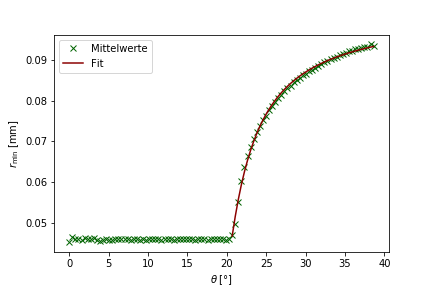
\includegraphics[width=0.5\textwidth]{plots/rmin_mean_sim.pdf}
    \caption{Mittelwerte der $r_{\mathrm{min}}$ in Abhängigkeit vom Winkel $\theta$. }
    \label{fig:rmin_mean_sim}
\end{figure}
\FloatBarrier
Die $r_{\mathrm{min}}$-Werte weisen bis zu einem Winkel von $\theta \approx \SI{20}{°}$ einen konstanten Wert von etwa $\SI{45}{\micro m}$ auf und steigen anschließend an.
In den Anstieg wird eine Fit-Funktion der Form
\begin{align}
    r_{\mathrm{min}}(\theta) = a \arctan(b + c \theta)
\end{align}
gelegt.
-------------Warum diese Funktion?----------
Mittels der Funktion \textit{curve\_fit} des Packetes \textit{scipy\_optimize} werden für die Parameter die Werte
\begin{align*}
    a = (655 \pm 2)\cdot 10^{-4} ,\\
    b = (-6.5 \pm 0.2),\\
    c = (358 \pm 9)\cdot 10^{-3}
\end{align*}
ermittelt.

Aus Abbildung \ref{fig:Hist_rmin_sim} wird außerdem der maximale Winkel bestimmt, unter welchem Kernphotonen die Ausleseelektronik erreichen. Hierzu wird in Abhängigkeit vom minimalen Abstand $r_{\mathrm{min}}$ der Winkel bestimmt, ab welchem weniger als 130 Einträge in einem Bin vorhanden sind. Die Grenzwinkel $\theta_{\mathrm{max}}$ sind in Abbildung \ref{fig:theta_max_sim} gegen $r_{\mathrm{min}}$ aufgetragen.
\begin{figure}
    \centering
    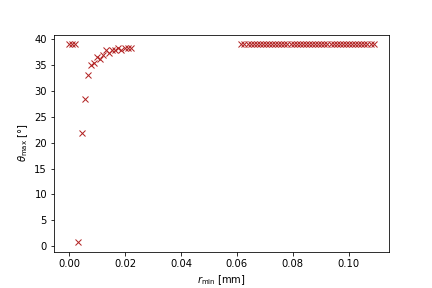
\includegraphics[width=0.5\textwidth]{plots/theta_max_sim.pdf}
    \caption{Grenzwinkel $\theta_{\mathrm{max}}$, unter welchem Photonen noch detektiert werden, in Abhängigkeit vom minimalen Abstand zur Faserlängsachse $r_{\mathrm{min}}$. }
    \label{fig:theta_max_sim}
\end{figure}
\FloatBarrier
-------------Plot noch sinnvoller machen----------\\


Des Weiteren werden die Reflektionswinkel $\theta_{\mathrm{refl}}$ nach Gleichung \eqref{eq:2} berechnet und ihre Verteilung in Abbildung \ref{fig:Theta_refl_sim} in Abhängigkeit vom Winkel $\theta$ aufgetragen.
\begin{figure}
    \centering
    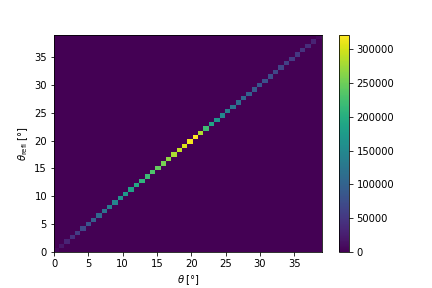
\includegraphics[width=0.5\textwidth]{plots/Theta_refl_sim.pdf}
    \caption{Verteilung der Reflektionswinkel $\theta_{\mathrm{refl}}$ in Abhängigkeit vom Winkel $\theta$. }
    \label{fig:Theta_refl_sim}
\end{figure}
\FloatBarrier
Analog zu den minimalen Abständen $r_{\mathrm{min}}$ werden die Mittelwerte des Reflektionswinkel pro Winkel $\theta$ bestimmt und in Abbildung \ref{fig:Theta_refl_mean_sim} in Abhängigkeit von $\theta$ dargestellt.
\begin{figure}
    \centering
    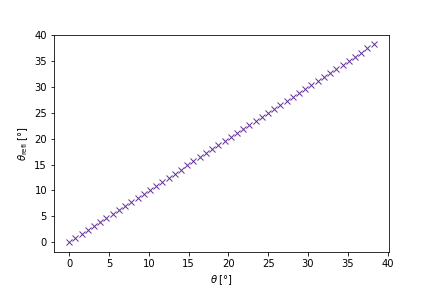
\includegraphics[width=0.5\textwidth]{plots/Theta_refl_mean_sim.pdf}
    \caption{Mittelwerte der Reflektionswinkel $\theta_{\mathrm{refl}}$ in Abhängigkeit vom Winkel $\theta$. }
    \label{fig:Theta_refl_mean_sim}
\end{figure}
\FloatBarrier
Es zeigt sich ein linearer Zusammenhang zwischen dem Reflektionswinkel $\theta_{\mathrm{refl}}$ und dem Winkel des Photons zur Faserachse $\theta$.
